\scanpage{16}
\[
\left\{\begin{aligned}
f_1&=(1,\unsure{\zeta|\xi},0)=e_1+\zeta e_2\\
f_2&=(1,0,1-\zeta)=e_1+(1-\zeta)\deleted{\unsure{f_3}}e_3
\deleted{=\underbrace{(0,\unsure{\zeta},\unsure{\zeta-1})}_{\text{vecteur directeur de la }2^{\mathrm e}\text{ droite isotrope}}=e_2+(\zeta-1)e_3}\\
f_3&=(0,0,1)=e_3
\end{aligned}\right.
\]
\figure{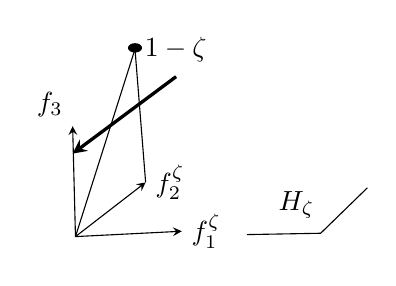
\begin{tikzpicture}[x=.9cm,y=.85cm,>=stealth]
\draw[->] (0,0)--(1.5,.08) node[right] {$f_1^\zeta$};
\draw[->] (0,0)--(.99,.81) node[right] {$f_2^\zeta$};
\draw[->] (0,0)--(-.04,1.65) node[above left] {$f_3$};
\fill (.84,2.82) ellipse (.10 and .07);
\draw (.99,.81)--(.84,2.8) node[right] {\unsure{$1-\zeta$}};
\draw (0,0)--(.84,2.8);
\draw[->,very thick] (1.42,2.39)--(-.04,1.24);
\draw (2.42,.03)--(3.46,.05)--(4.12,.73);
\node at (3.12,.47) {$H_\zeta$};
\end{tikzpicture}}

\uline{NB}
\[
\begin{aligned}
e_1&=f_2-(1-\zeta)f_3=f_2+(\zeta-1)f_3\\
e_2&=\zeta^{-1}(f_1-e_1)=\zeta^{-1}f_1-\zeta^{-1}f_2+(1-\zeta^{-1})f_3\\
e_3&=f_2\\
&\deleted{\unsure{f_2}=\zeta^{-1}f_1\unsure{-}\zeta^{-1}f_2+(1-\zeta^{-1})f_3}
\end{aligned}
\]
Le plan \inserted{$(e_1,e_2)$ est \unsure{insécable|invariable|invariant} !} engendré par $(f_1,e_1)$ (qui correspond à la droite isotrope $D_{\zeta^{-1}}=D'_\zeta\ldots$), qui correspond dans le plan $(f_2,f_3)$ -- (si $\zeta-1$ inv.) à la droite de pente (p.r. à $f_3,f_2$) $\dfrac{1}{\zeta-1}$

\medskip
\deleted{Donnée du Polygone épinglé \inserted{\unsure{pointé|par $\infty$|par $D_\zeta$}} de type $\ne\mathrm{III}$ \deleted{équivaut}\inserted{\unsure{i.e. est équiv|i.e. est ép|i.e. réguliers}} $+$ droite isotrope $\Longleftrightarrow$ donnée de $\zeta\in\Gamma(S,\underline O_S)^*$ $\Longleftrightarrow$ ce qui suit :}

\deleted{1°) fibré \deleted{en droites affines \unsure{$F$} sur $S$ i.e. \unsure{torseur sous|disons un|torseurs sous}} fibré vectoriel \inserted{de rang $1$} \deleted{inv. \unsure{$F$} i.e. est en lien \unsure{$V$|via}}\inserted{$F$} lié par un $L$}

\[
\deleted{0-L-F-\underline O_S\longrightarrow0}
\]
\deleted{2°) Une section de $\mathbb P(F)$ i.e. un Module inv. $L'$ et un hom}
\[
\deleted{F\longrightarrow L'}
\]
Avec ceci, on construit le schéma en groupes
% archive sheet number: 15
